\documentclass[12pt]{amsart}
\usepackage{epigraph}
\usepackage[]{filecontents}
\usepackage[]{lettrine}
\usepackage[]{graphicx}
\usepackage[]{listings}
\usepackage[]{xcolor}
\usepackage[]{biblatex}
\usepackage[]{hyperref}

\setlength\epigraphwidth{10cm}

\lstdefinelanguage{Maple}% 
{morekeywords={and,assuming,break,by,catch,description,do,done,% 
elif,else,end,error,export,fi,finally,for,from,global,if,% 
implies,in,intersect,local,minus,mod,module,next,not,od,% 
option,options,or,proc,quit,read,return,save,stop,subset,then,% 
to,try,union,use,uses,while,xor,RETURN},% 
sensitive=true,% 
morecomment=[l]\#,% 
morestring=[d]{"'`},% 
morestring=[d]"% 
}[keywords,comments,strings]% 

% See: https://en.wikibooks.org/wiki/LaTeX/Source_Code_Listings
\lstdefinestyle{maple}{
  belowcaptionskip=1\baselineskip,
  breaklines=true,
  frame=single,
  language=Maple,
  xleftmargin=\parindent,
  showstringspaces=false,
  basicstyle=\small\ttfamily,
  keywordstyle=\bfseries\color{green!60!black},
  commentstyle=\itshape\color{purple!40!black},
  identifierstyle=\color{black},
  stringstyle=\color{orange},
}

\lstset{escapechar=@,style=maple, numbers=left}

\begin{filecontents}{cite.bib}
@book{hargrave,
  title={{A History of Playing Cards and a Bibliography of Cards and Gaming}},
  author={Hargrave, Catherine Perry},
  year={2000},
  publisher={Courier Corporation}
}
\end{filecontents}

\addbibresource{cite.bib}

\title{The Game of War}
\author{Alison Bu, Robert Dougherty-Bliss, Charles Kenney}
\date{\today}


\begin{document}


\maketitle


\epigraph{\emph{Primitive man tossed his arrows into the magic ring which he had
    drawn on the ground with the proper rites and incantations. And who can say
    that some power higher than the stars did not direct their flight, and
bring him in safety to his journey's end?}}{--- Catherine Hargrave, \emph{A History of Playing Cards}}

\section{Introduction}%
\label{sec:introduction}

\lettrine[lraise=0.16]{W}{e, the war team,} were assigned to study the game of
War, a classic, internationally-known card game. To this end, we have written a
comprehensive collection of Maple code to simulate and analyze War and various
generalizations we have considered.

The main items of our report are as follows:

\begin{itemize}
    \item A large body of Maple code.
    \item Pictures of the ``War graph'' for small hands.
    \item A definition of the sequence, ``longest possible game of War on the
        deck $[n] = \{1, 2, \dots, n\}$.''
\end{itemize}

Our report is structured into three parts. Section~\ref{sec:history} contains
our (failed) attempt to reconstruct the history of War\footnotemark.
Section~\ref{sec:procedures} contains all of our Maple code.
Section~\ref{sec:graph} contains some notes on the ``War graph'' as well as
some pictures we made.

\footnotetext{The game, of course.}

\section{A History of Cards}
\label{sec:history}

% I don't know why I'm writing this section, really. It just seemed interesting,
% and I couldn't find anything about the history of war.


% Not a very convincing paragraph.


The game of war seems nearly universal. In America, we play \emph{War}; in
England, they call it \emph{Battle}; the Germans have a varient called
\emph{Tod und Leben}. Despite its popularity, the origins of War are completely
mysterious. There are references to \emph{Tod und Leben} found in nineteenth
century game books, but surely the game of war existed before this in different
forms. Lacking any authoritative history on the subject, it seems just as good
to talk about the history of playing cards themselves, and perhaps surmise when
War \emph{could} have been invented based on this.

Playing cards have surely existed in some form for much longer than we have
records of them. Stewart Culin, the great American game expert and early
ethnographer, believed that playing cards descended from divination rituals,
which existed in nearly every culture around the world: ``In order to classify
objects and events which did not in themselves reveal their proper assignment,
resort was had to magic. Our present games are the survivals of these magical
processes'' \cite[p.~1]{hargrave}.

Nonetheless, the earliest \emph{known} playing cards are Chinese and from the
twelfth century. The cards were copied from Chinese notes invented in the Tang
Dynasty (est.~618 CE)--- gamblers likely played with the notes themselves.
Other popular cards, used interchangeably, were \emph{domino cards}, cards with
patterns of dots added for significance. These are quite beautiful---see
Figure~\ref{fig:domino}.

\begin{figure}[htpb]
    \centering
    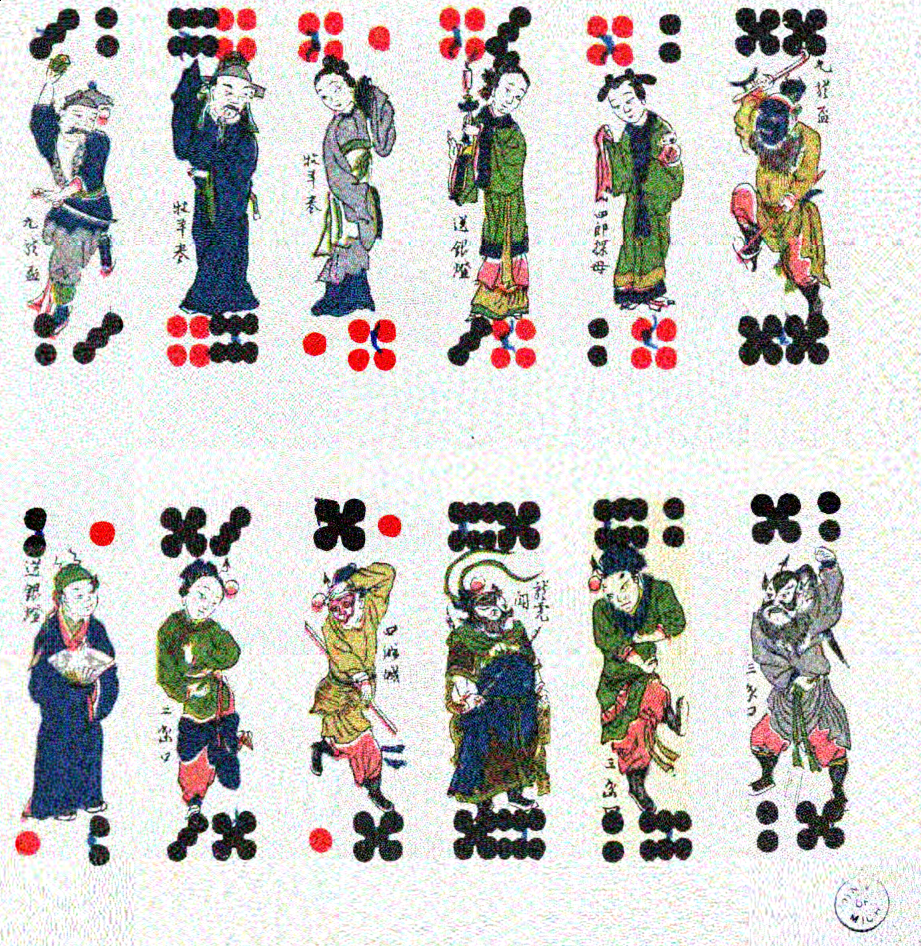
\includegraphics[width=0.8\linewidth]{domino}
    \caption{Chinese domino cards depicting characters from the story of the
    river banks. From \cite{hargrave}.}
    \label{fig:domino}
\end{figure}


It is unclear how or in what form playing cards first spread to Europe. One
popular theory asserts that ``wandering gypsies'' brought them from India.
Culin believed the opposite, that Indian playing cards were inspired by early
European developments. However they arrived, the modern playing card was
developed in France.


The first French playing cards were tarot cards---still available
today---painted for King Charles VI in 1392 CE, and popular among
working-people no later than 1397 CE. Tarot cards come in collections of
twenty-two, painted with figures and scenes which hold some significance, such
as \emph{Le bateleur} (``The magician''), \emph{Le chariot}, and \emph{La
justice}. The cards begin with suites of Cups, Swords, Coins, and Batons, but
were changed to Hearts, Clubs, Spades, and Diamonds when, according to legend,
the famous Hundred Years' War commander La Hire invented the game of piquet. At
this time the cards were numbered linearly \emph{by suite}. Around 1440, the
first ``court'' (face) cards were named. By 1516 the standard 52-card deck had
been invented. These are essentially the cards that we still use today, some
half-a-millennium later.

In summary, playing cards with numeric values have been around for hundreds of
years. Some of the earliest games we have records of are already more
complicated than War. It seems difficult to pinpoint exactly when the game
started, but it must have been well-over two-hundred years ago, if not
\emph{significantly} further in our history.


\section{Procedures}
\label{sec:procedures}
\subsection{Setting Up the Game}


\subsubsection{Distributing the Deck} \hfill


The procedure \textbf{RanDeck(n,k,r)} inputs positive integers $n,k,$ and $r$. It simulates dealing out a randomly shuffled deck of cards containing $k$ copies of $n$ unique, ordered cards to $r$ players.\footnote{In other words, $kn$ cards with $k$ suits.}
 The maximal number of cards such that each player has the same number of cards are dealt out and any remaining cards are removed from the game.


\textbf{RanDeck(n,k,r)} partitions the first $\lfloor\frac{n*k}{r}\rfloor *r $ entries of a random permutation of $[ \underbrace{1,...,1}_{r \text{ copies}},...,\underbrace{n,...,n}_{r \text{ copies}}]$ by creating a new part after every $\lfloor \frac{n*k}{r} \rfloor$-th entry. It outputs this partition as a list of length $r$, where the $i$-th entry is a list that represents the $i$-th players deck.


\begin{lstlisting}
RanDeck:=proc(n,k,r) local HandSize, i, pi, Deck, decks, discard:
 Deck:=[seq(seq(i,j=1..k),i=1..n)]:
 Deck:=randperm(Deck):
 HandSize:=floor(n*k/r):
 decks:=[seq([seq(Deck[i],i=(j-1)*HandSize+1..j*HandSize)],j=1..r)]:
 end:
\end{lstlisting}


\subsubsection{Defining War}\hfill


A war occurs when the highest card played in a round is not unique. In a war, players place $m$ cards face down and then play their next card. The following three procedures define different ways to complete a war when a player does not have enough cards.  Each of the following procedures input a non-negative integer $m$, a list $Q$, and a positive integer $r$, where $Q[i]$ represents the $i$-th player's deck and $|Q|=r$.


The procedure \textbf{WARm(m,Q,r)} simulates a war where $m$ cards must be placed face down, and any player that does not have enough cards automatically loses. If no player has enough cards to complete the war, it outputs $\{0\}$ to indicate that the game will have no winners. Otherwise, it outputs a list $[tempQ,b]$, where $tempQ$ is a list of each players deck after placing $m$ cards face down and $b$ is a list of the cards placed face down or played during the war.


\begin{lstlisting}
WARm:=proc(m,Q,r) local HandSize, tempQ,i,output,a,b:
  HandSize:=[seq(nops(Q[i]), i=1..r)]:
  if max(HandSize)>m then tempQ:=Q: a:=Q:
  for i from 1 to r do 
    if HandSize[i]<m+1 then tempQ[i]:=[]:  a[i]:=[op(1..-1,Q[i]),seq(0,j=HandSize[i]..m)]: 
    else tempQ[i]:=[op(m+1..-1,Q[i])]: a[i]:=[op(1..m,Q[i])]: 
    fi: od: 
  b:=remove(t->t=0,[seq(seq(a[i][j],i=1..r),j=1..m)]):
  output:=[tempQ,b]:
  else output:={0}: fi:
  output:
 end:
\end{lstlisting}




The procedure \textbf{WARmin(m,Q,r)} inputs a non-negative integer $m$, a list $Q$, and a positive integer $r$ such that $|Q|=r$.  It simulates a war where $Q[i]$ represents the $i$-th player's deck, and $m$ cards must be placed face down unless any player still in the game does not have enough cards to do so.  If the smallest hand at the start of the war is $k<m+1$, then every player places $k-1$ cards face down and plays their next card.  If no player has any remaining cards, it outputs 0 to indicate that the game will end in a tie. Otherwise, it outputs a list $[tempQ,b]$, where $tempQ$ is a list of each players deck after placing their cards face down and $b$ is a list of the cards placed face down or played during the war.


\begin{lstlisting}
WARmin:=proc(m,Q,r) local HandSize, hs, tempQ,i,output:
  HandSize:=[seq(nops(Q[i]),i=1..r)]
  if add(HandSize[i],i=1..r)<1 then output:=0:
  else hs:=min(remove(t->t=0,HandSize)):
    if hs>m then output:=WARm(m,Q,r):
    else output:=WARm(hs-1,Q,r):
    fi:
  fi:  
  output:
 end:
\end{lstlisting}




The procedure \textbf{WARmax(m,Q,r)} inputs a non-negative integer $m$, a list $Q$, and a positive integer $r$ such that $|Q|=r$.  It simulates a war where the $i$-th entry of $Q$ represents the $i$-th player's deck, and $m$ cards must be placed face down unless no player still in the game has enough cards to do so.  If the largest hand at the start of the war is $k<m+1$, then every player places $k-1$ cards face down and plays their next card. Any player that does not have nough cards to do so automatically loses.  If no player has any remaining cards, it outputs 0 to indicate that the game will end in a tie. Otherwise, it outputs a list $[tempQ,b]$, where $tempQ$ is a list of each players deck after placing their cards face down and $b$ is a list of the cards placed face down or played during the war.


\begin{lstlisting}
WARmax:=proc(m,Q,r) local HandSize,HS, tempQ,i,output:
  HandSize:=[seq(nops(Q[i]),i=1..r)]:
  HS:=max(HandSize):
  if HS>m then output:=WARm(m,Q,r):
   elif HS=0 then output:=0:
   else output:=WARm(HS-1,Q,r):
   fi:
  output:
end: 
\end{lstlisting}




\subsubsection{Defining Replacement}\hfill


The following procedures define how cards are placed back into the deck after winning a round. Each procedure inputs a list $Q$, a positive integer $r$ where $|Q|=r$, a list $b$, and a positive integer $N$. The $i$-th entry of $Q$ represents the $i$-th player's deck, $b$ lists the cards on the table in the order they were played where Player $i$ is the $i$-th player to play a card (i.e. $b$ lists the cards that the winner of the round will take), and Player $N$ is the winner of the round.


The procedure \textbf{RepPlayed(Q,r,b,N)} outputs a list of each players hand after adding the won cards to the bottom of Player $N$'s deck in the order that they were played.


\begin{lstlisting}
RepPlayed:=proc(Q,r,b,N) local c:
  c:=remove(t->t=0,b):
  [seq(Q[i],i=1..N-1),[op(Q[N]),op(c)],seq(Q[i],i=N+1..r)]:
 end:
\end{lstlisting}


The procedure \textbf{RepAllAsc(Q,r,b,N)} outputs a list of each players hand after sorting all the won cards in ascending order and then placing them at the bottom of Player $N$'s deck.


\begin{lstlisting}
RepAllAsc:=proc(Q,r,b,N) local c:
  c:=remove(t->t=0,b):
  c:=sort(c):
  [seq(Q[i],i=1..N-1),[op(Q[N]),op(c)],seq(Q[i],i=N+1..r)]:
end:
\end{lstlisting}


The procedure \textbf{RepAllDesc(Q,r,b,N)} outputs a list of each players hand after sorting all the won cards in descending order and then placing them at the bottom of Player $N$'s deck.




\begin{lstlisting}
RepAllDesc:=proc(Q,r,b,N) local c:
  c:=remove(t->t=0,b):
  c:=sort(b,`>`):
  [seq(Q[i],i=1..N-1),[op(Q[N]),op(c)],seq(Q[i],i=N+1..r)]:
end:
\end{lstlisting}




The procedure \textbf{RepAsc(Q,r,b,N)} outputs a list of each players hand after sorting each subround (i.e. each time all the players placed a card on the table) in ascending order and then placing them at the bottom of Player N's deck. In a war, the cards that each player placed face down first are sorted in ascending order, then then the card that each player put down next are sorted in ascending order, and so on.




\begin{lstlisting}
RepAsc:=proc(Q,r,b,N) local n,c:
  n:=nops(b)/r:
  c:=[seq(op(sort([op(i*r+1..i*r+r,b)])),i=0..n-1)]:
  c:=remove(t->t=0,c):
  [seq(Q[i],i=1..N-1),[op(Q[N]),op(c)],seq(Q[i],i=N+1..r)]:
end:
\end{lstlisting}


The procedure \textbf{RepDesc(Q,r,b,N)} outputs a list of each players hand after sorting each subround (i.e. each time all the players placed a card on the table) in descending order and then placing them at the bottom of Player N's deck.




\begin{lstlisting}
RepDesc:=proc(Q,r,b,N) local n,c:
  n:=nops(b)/r:
  c:=[seq(op(sort([op(i*r+1..i*r+r,b)],`>`)),i=0..n-1)]:
  c:=remove(t->t=0,c):
  [seq(Q[i],i=1..N-1),[op(Q[N]),op(c)],seq(Q[i],i=N+1..r)]:
end:
\end{lstlisting}




\subsection{Simulating a Game of War}


\subsubsection{Simulating One Move or Round}\hfill


The procedure \textbf{OneMove(P,c,m,WAR,rep)} inputs a list $P$, a list $c$, a positive integer $m$, a war procedure WAR, and a replacement procedure rep. The $i$-th entry of $P$ is a list representing the $i$-th player's hand at the beginning of the move, $c$ lists the cards that have already been placed on the table during this round (i.e. cards accumulated during unresolved wars), and $m$ is the default number of cards to be placed face down during a war. If this round ends the game with no winners it outputs $\{0\}$. If the round ends the game with a tie, then it outputs a set of the players that tied. Otherwise, it outputs a list $Q$ where the $i$-th entry represents each players deck at the end of the round after adding the won cards to the bottom of the winner's deck.


\textbf{OneMove(P,c,m,WAR,rep)} adds $0$ to any empty deck to represent no card, then creates a list $a$ of the first card of each player's deck and a new list $Q$ where the $i$-th entry of $Q$ represents each player's deck after removing their first card. It finds the highest value in $a$ and checks if any other player's had the same card. If the highest card was unique, it places all of the cards at the bottom of the winners deck according to rep. Otherwise, it runs WAR(m,Q,r) to simulate a war. If player's are able to play a card after placing cards face down on the table, it runs $OneMove(Q,b,m,WAR,rep)$ where $Q$ and $b$ are lists such that the $i$-th entry of $Q$ represents the $i$-th player's deck after placing cards on the table, and $b$ lists the cards that have already been placed on the table during this round.


\begin{lstlisting}
OneMove:=proc(P,c,m,WAR,rep) local r, a, b, tempP, i, h, w, Q, output, W:
  r:=nops(P):
  a:=[]:
  b:=[op(c)]:
  tempP:=P:
  for i from 1 to r do
    if P[i]=[] then tempP[i]:=[0]: fi: od:
  a:=[seq(tempP[i][1],i=1..r)]:
  Q:=[seq([op(2..-1,tempP[j])],j=1..r)]:
  h:=max(op(a)):
  w:={SearchAll(h,a)}:
  if nops(w)=1 then
    b:=[op(b),op(a)]:
    output:=rep(Q,r,b,op(w)): 
  else
    W:=WAR(m,Q,r):
    if type(W,list)=true then
      Q:=W[1]:
      b:=[op(b),op(a),op(W[2])]: 
     output:=OneMove(Q,b,m, WAR,rep):
     elif type(W,integer)=true then
       output:=tie:
     else
       output:=W:
     fi: fi:
  output:
  end:
\end{lstlisting}


\subsection{The War Graph: Procedures}
The procedures \textbf{WarGraph(n)} and \textbf{ArbRelWG(M)} (short for "arbitrary-relation war graph")
use the GraphTheory package in Maple to construct the \emph{game graph} of war.
In WarGraph, the game is played with a simple $n$-card deck $\{1,2,...,n\}$; when players skirmish,
the winner is always the player of the higher card, and the winner of the game (if there is any) is always the player who began the game with the high-card $n$. For this reason, we have ``modded out" by the symmetry
of exchanging the two players' hands, and allowed only the hands in which the left player Leftie holds the card $n$. 
A position in War--a pair of players' hands $[[L_1, L_2,...,L_m],[R_1,R_2,...,R_\ell]]$--is called \emph{terminal}
if one player (for us, always the right player Rita) has an empty hand $[]$. Apart from terminal positions,
every position in simple War\footnote{That is, war with two players on the linearly ordered deck $\{1,...,n\}$} has two ``children" (two positions that could result from playing one Skirmish), and \textbf{ChildLW} and \textbf{ChildWL} record these two possibilities. The player who wins the skirmish must put the two cards at the bottom of their deck, and there are two possible orders in which to do this, LW (losing-winning) and WL (winning-losing). For example, here is ChildWL:
\begin{lstlisting}
ChildWL:=proc(Hands):
if nops(Hands[1])>0 and nops(Hands[2])>0 then


if Hands[1][1] > Hands[2][1] then
[[op(Hands[1][2..]),Hands[1][1],Hands[2][1]],Hands[2][2..]]:
else
[Hands[1][2..], [op(Hands[2][2..]),Hands[2][1],Hands[1][1]]]:
fi:


else
Hands:
fi:
end:
\end{lstlisting}
The WarGraph is the directed graph in which each node is a position, and directed edges are introduced
from each position to its possible children. It was first studied in Lakshtanov and Roshchina 2011. Here is the code:
\begin{lstlisting}
WarGraph:=proc(n) local positions,perms,i,G,p,splits,H,spot,V,v,S,s,U:
perms:=permute(n): 


positions:=[]:


for p in perms do
 spot:=Search(n,p):
 splits:=seq(convert([p[..i],p[i+1..]],string),i=spot..n):
 positions:=[op(positions),splits]:
od:


G:=Digraph(positions):


for H in positions do
 H:=parse(H):


if nops(H[1]) = 0 or nops(H[2]) = 0 then
else
AddArc(G,{[convert(H,string),convert(ChildWL(H),string)],
[convert(H,string),convert(ChildLW(H),string)]}):
fi:
od:


G:
end:
\end{lstlisting}
See also the War Graph section. 


ArbRelWG is a generalization of WarGraph, in which the winners of skirmishes is determined by
the matrix $M$, rather than standard comparison. The matrix $M$ consists of $0$s and $1$s,
with the rule
$$M[i][j] = \begin{cases} 1 \ \text{if card} \ i \ \text{beats card} \ j \\ 0 \ \text{else.} \end{cases} $$
For example, $M$ could encode the rock-paper-scissors deck:
$$M = \begin{pmatrix} 0 & 0 & 1 \\ 1 & 0 & 0 \\ 0 & 1 & 0 \end{pmatrix}.$$
The procedures ArbRelChildLW and ArbRelChildWL are the analogs of ChildLW and ChildWL
for this generalized version of War. The two major differences between ArbRelWG
and WarGraph are: (1) there is now no notion of a ``high card," so the entire set of $(n+1)!$
positions show up as vertices, and (2) winners are now determined by appeal to the matrix $M$, as you will see:


\begin{lstlisting}
ArbRelWG:=proc(M) local n, positions,perms,i,G,p,splits,H,spot,V,v,S,s,U:
n:=nops(M):


perms:=permute(n): 


positions:=[]:


for p in perms do
splits:=seq(convert([p[..i],p[i+1..]],string),i=0..n):
positions:=[op(positions),splits]:
od:


G:=Digraph(positions):


for H in positions do
H:=parse(H):


if nops(H[1]) = 0 or nops(H[2]) = 0 then
else
 AddArc(G,{[convert(H,string),convert(ArbRelChildWL(H,M),string)],
[convert(H,string),convert(ArbRelChildLW(H,M),string)]}):
fi:
od:


G:
end:
\end{lstlisting}


\section{The War Graph}
\label{sec:graph}

\clearpage

\printbibliography



\end{document}
